\section{Segnalazione errori}
Nel caso si riscontrassero anomalie o errori durante l'esecuzione del plug-in o dell'applicazione di addestramento, è possibile segnalarli tramite l'indirizzo email {\url{vram.software@gmail.com}}.
	\subsection{Segnalazione errori nell'applicazione di addestramento}
	Indicare nell'oggetto [BUG][AppAddestramento] se si vuole segnalare la presenza di un bug nell'applicazione di addestramento.
	Nel corpo della mail indicare:
	\begin{itemize}
		\item versione dell'applicazione di addestramento;
		\item sistema operativo e relativa versione;
		\item descrizione dettagliata dell'errore riscontrato.
	\end{itemize}
	\mbox{}
	\begin{figure} [H]
		\begin{center}
			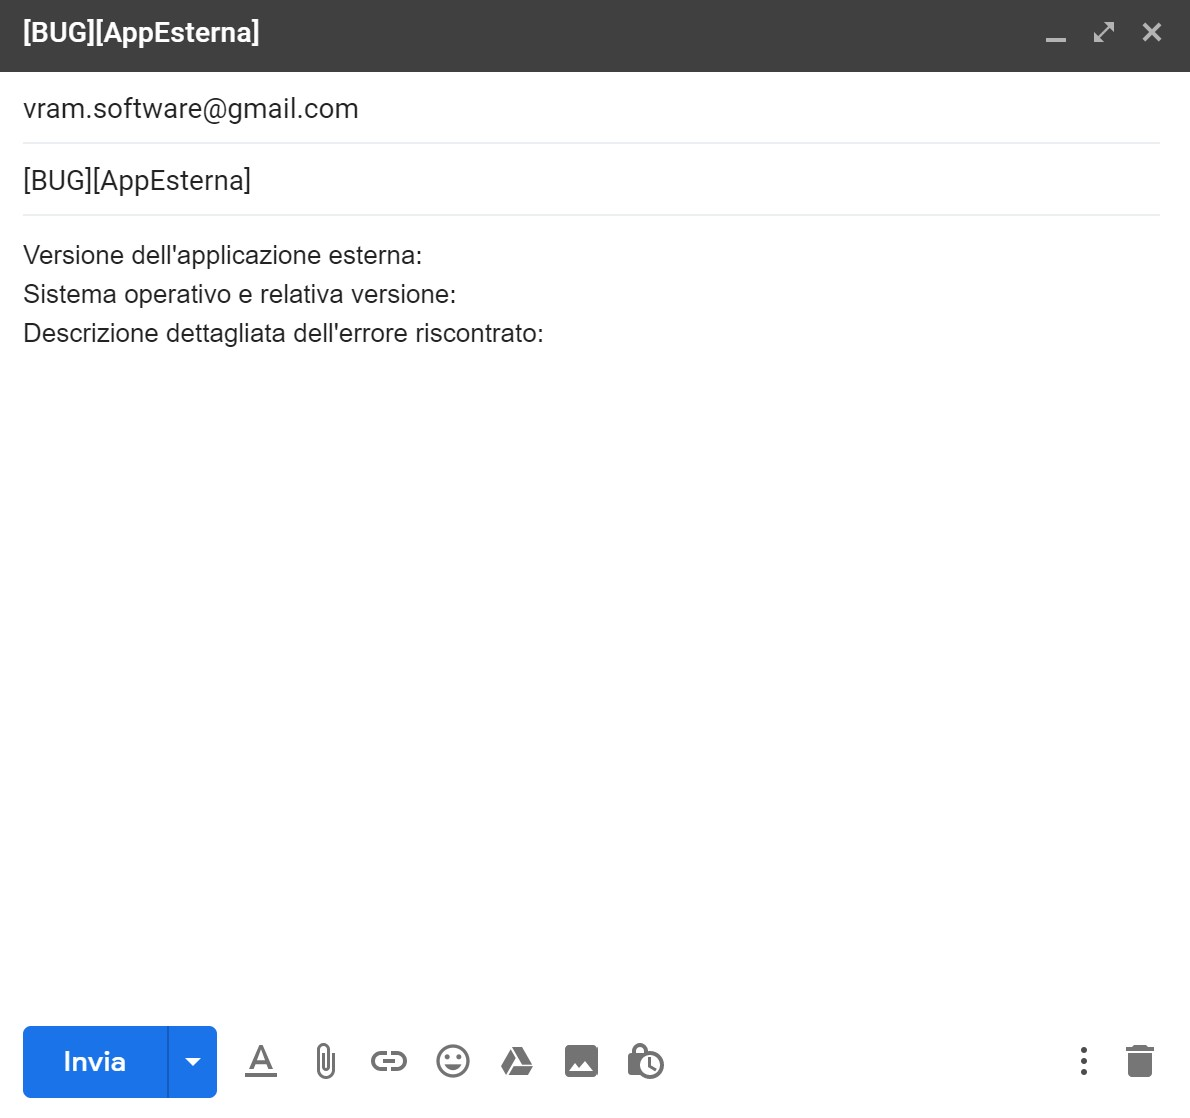
\includegraphics[width=120mm]{./img/erroriApp.jpg}
		\end{center}
		\caption{Template email segnalazione errori nell'applicazione di addestramento}
	\end{figure}
	\mbox{}
	\subsection{Segnalazione errori nel plug-in}
 	[BUG][Plug-in] se si vuole segnalare la presenza di un bug nel plug-in.
 	Nel corpo della mail indicare:
 	\begin{itemize}
 		\item versione del plug-in;
 		\item versione di Grafana\glo;
 		\item sistema operativo e relativa versione;
 		\item browser utilizzato e relativa versione;
 		\item descrizione dettagliata dell'errore riscontrato.
 	\end{itemize}
 	\mbox{}
 	\begin{figure} [H]
 		\begin{center}
 			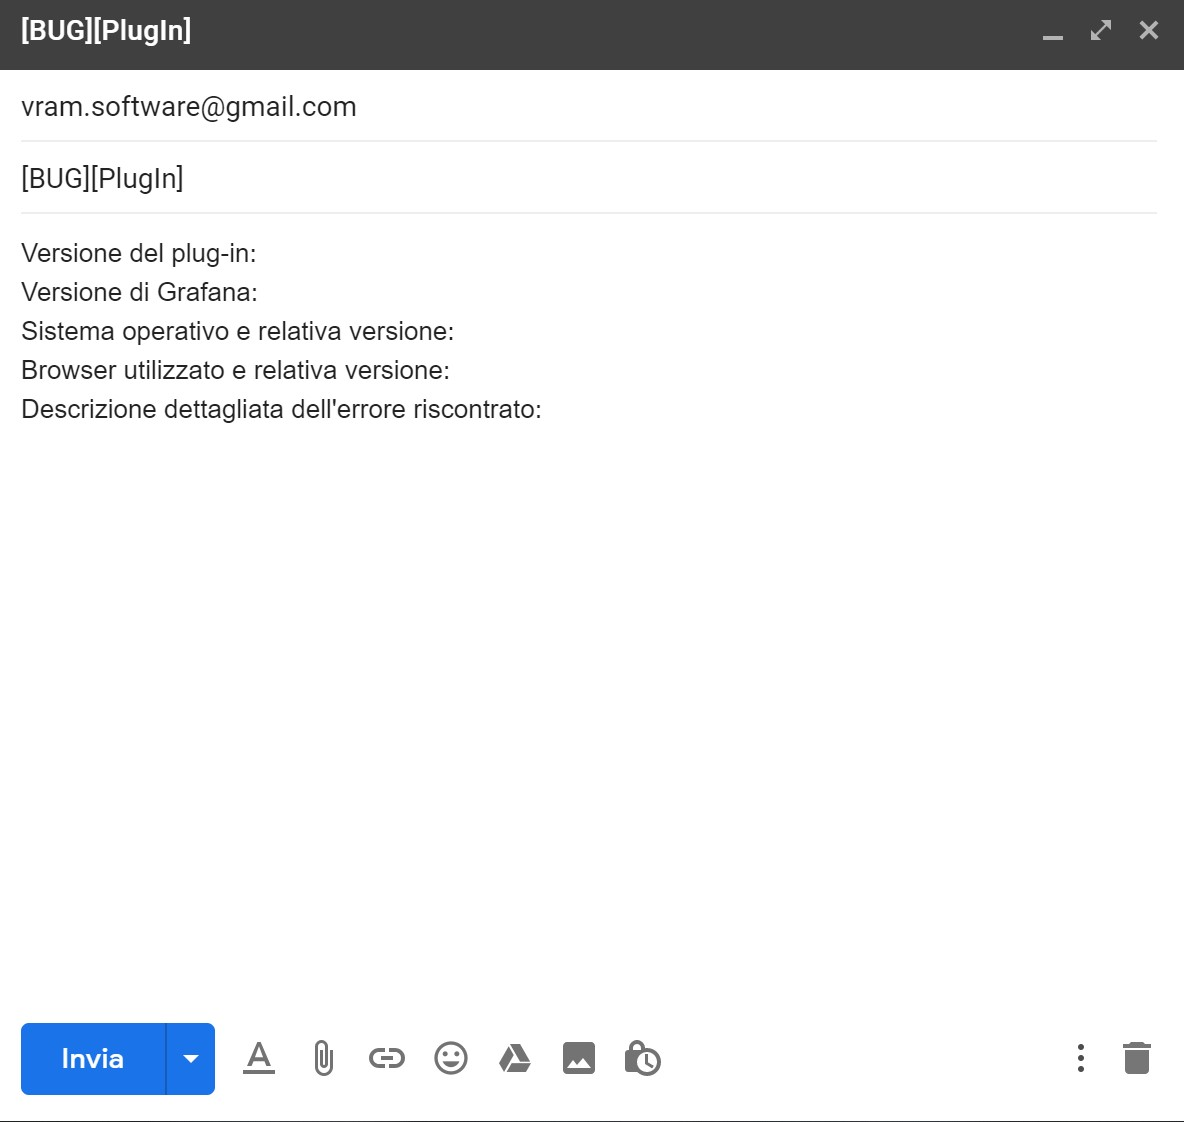
\includegraphics[width=120mm]{./img/erroriPlugIn.jpg}
 		\end{center}
 		\caption{Template email segnalazione errori nel plug-in}
 	\end{figure}
